
\documentclass[letterpaper,hide notes,xcolor={table,svgnames},pdftex,10pt]{beamer}
\def\showexamples{t}


%\usepackage[svgnames]{xcolor}

%% Demo talk
%\documentclass[letterpaper,notes=show]{beamer}

\usecolortheme{crane}
\setbeamertemplate{navigation symbols}{}

\usetheme{MyPittsburgh}
%\usetheme{Frankfurt}

%\usepackage{tipa}

\usepackage{hyperref}
\usepackage{graphicx,xspace}
\usepackage[normalem]{ulem}
\usepackage{multicol}
\usepackage{amsmath,amssymb,amsthm,graphicx,xspace}
\newcommand\SF[1]{$\bigstar$\footnote{SF: #1}}

\usepackage[default]{sourcesanspro}
\usepackage[T1]{fontenc}
\usepackage[scaled]{beramono}
\usepackage{tikzpagenodes}

\newcounter{tmpnumSlide}
\newcounter{tmpnumNote}


% old question code
%\newcommand\question[1]{{$\bigstar$ \small \onlySlide{2}{#1}}}
% \newcommand\nquestion[1]{\ifdefined \presentationonly \textcircled{?} \fi \note{\par{\Large \textbf{?}} #1}}
% \newcommand\nanswer[1]{\note{\par{\Large \textbf{A}} #1}}


 \newcommand\mnote[1]{%
   \addtocounter{tmpnumSlide}{1}
   \ifdefined\showcues {~\tiny\fbox{\arabic{tmpnumSlide}}}\fi
   \note{\setlength{\parskip}{1ex}\addtocounter{tmpnumNote}{1}\textbf{\Large \arabic{tmpnumNote}:} {#1\par}}}

\newcommand\mmnote[1]{\note{\setlength{\parskip}{1ex}#1\par}}

%\newcommand\mnote[2][]{\ifdefined\handoutwithnotes {~\tiny\fbox{#1}}\fi
% \note{\setlength{\parskip}{1ex}\textbf{\Large #1:} #2\par}}

%\newcommand\mnote[2][]{{\tiny\fbox{#1}} \note{\setlength{\parskip}{1ex}\textbf{\Large #1:} #2\par}}

\newcommand\mquestion[2]{{~\color{red}\fbox{?}}\note{\setlength{\parskip}{1ex}\par{\Large \textbf{?}} #1} \note{\setlength{\parskip}{1ex}\par{\Large \textbf{A}} #2\par}\ifdefined \presentationonly \pause \fi}

\newcommand\blackboard[1]{%
\ifdefined   \showblackboard
  {#1}
  \else {\begin{center} \fbox{\colorbox{blue!30}{%
         \begin{minipage}{.95\linewidth}%
           \hspace{\stretch{1}} Some space intentionally left blank; done at the blackboard.%
         \end{minipage}}}\end{center}}%
         \fi%
}



%\newcommand\q{\tikz \node[thick,color=black,shape=circle]{?};}
%\newcommand\q{\ifdefined \presentationonly \textcircled{?} \fi}

\usepackage{listings}
\lstset{basicstyle=\footnotesize\ttfamily,
	breaklines=true,
	aboveskip=15pt,
  	belowskip=15pt,
	frame=lines,
	numbers=left, basicstyle=\scriptsize, numberstyle=\tiny, stepnumber=0, numbersep=2pt
}

\usepackage{siunitx}
\newcommand\sius[1]{\num[group-separator = {,}]{#1}\si{\micro\second}}
\newcommand\sims[1]{\num[group-separator = {,}]{#1}\si{\milli\second}}
\newcommand\sins[1]{\num[group-separator = {,}]{#1}\si{\nano\second}}
\sisetup{group-separator = {,}, group-digits = true}

%% -------------------- tikz --------------------
\usepackage{tikz}
\usetikzlibrary{positioning}
\usetikzlibrary{arrows,backgrounds,automata,decorations.shapes,decorations.pathmorphing,decorations.markings,decorations.text,decorations.pathreplacing}

\tikzstyle{place}=[circle,draw=blue!50,fill=blue!20,thick, inner sep=0pt,minimum size=6mm]
\tikzstyle{transition}=[rectangle,draw=black!50,fill=black!20,thick, inner sep=0pt,minimum size=4mm]

\tikzstyle{block}=[rectangle,draw=black, thick, inner sep=5pt]
\tikzstyle{bullet}=[circle,draw=black, fill=black, thin, inner sep=2pt]

\tikzstyle{pre}=[<-,shorten <=1pt,>=stealth',semithick]
\tikzstyle{post}=[->,shorten >=1pt,>=stealth',semithick]
\tikzstyle{bi}=[<->,shorten >=1pt,shorten <=1pt, >=stealth',semithick]

\tikzstyle{mut}=[-,>=stealth',semithick]

\tikzstyle{treereset}=[dashed,->, shorten >=1pt,>=stealth',thin]

\usepackage{ifmtarg}
\usepackage{xifthen}
\makeatletter
% new counter to now which frame it is within the sequence
\newcounter{multiframecounter}
% initialize buffer for previously used frame title
\gdef\lastframetitle{\textit{undefined}}
% new environment for a multi-frame
\newenvironment{multiframe}[1][]{%
\ifthenelse{\isempty{#1}}{%
% if no frame title was set via optional parameter,
% only increase sequence counter by 1
\addtocounter{multiframecounter}{1}%
}{%
% new frame title has been provided, thus
% reset sequence counter to 1 and buffer frame title for later use
\setcounter{multiframecounter}{1}%
\gdef\lastframetitle{#1}%
}%
% start conventional frame environment and
% automatically set frame title followed by sequence counter
\begin{frame}%
\frametitle{\lastframetitle~{\normalfont(\arabic{multiframecounter})}}%
}{%
\end{frame}%
}
\makeatother

\makeatletter
\newdimen\tu@tmpa%
\newdimen\ydiffl%
\newdimen\xdiffl%
\newcommand\ydiff[2]{%
    \coordinate (tmpnamea) at (#1);%
    \coordinate (tmpnameb) at (#2);%
    \pgfextracty{\tu@tmpa}{\pgfpointanchor{tmpnamea}{center}}%
    \pgfextracty{\ydiffl}{\pgfpointanchor{tmpnameb}{center}}%
    \advance\ydiffl by -\tu@tmpa%
}
\newcommand\xdiff[2]{%
    \coordinate (tmpnamea) at (#1);%
    \coordinate (tmpnameb) at (#2);%
    \pgfextractx{\tu@tmpa}{\pgfpointanchor{tmpnamea}{center}}%
    \pgfextractx{\xdiffl}{\pgfpointanchor{tmpnameb}{center}}%
    \advance\xdiffl by -\tu@tmpa%
}
\makeatother
\newcommand{\copyrightbox}[3][r]{%
\begin{tikzpicture}%
\node[inner sep=0pt,minimum size=2em](ciimage){#2};
\usefont{OT1}{phv}{n}{n}\fontsize{4}{4}\selectfont
\ydiff{ciimage.south}{ciimage.north}
\xdiff{ciimage.west}{ciimage.east}
\ifthenelse{\equal{#1}{r}}{%
\node[inner sep=0pt,right=1ex of ciimage.south east,anchor=north west,rotate=90]%
{\raggedleft\color{black!50}\parbox{\the\ydiffl}{\raggedright{}#3}};%
}{%
\ifthenelse{\equal{#1}{l}}{%
\node[inner sep=0pt,right=1ex of ciimage.south west,anchor=south west,rotate=90]%
{\raggedleft\color{black!50}\parbox{\the\ydiffl}{\raggedright{}#3}};%
}{%
\node[inner sep=0pt,below=1ex of ciimage.south west,anchor=north west]%
{\raggedleft\color{black!50}\parbox{\the\xdiffl}{\raggedright{}#3}};%
}
}
\end{tikzpicture}
}


%% --------------------

%\usepackage[excludeor]{everyhook}
%\PushPreHook{par}{\setbox0=\lastbox\llap{MUH}}\box0}

%\vspace*{\stretch{1}

%\setbox0=\lastbox \llap{\textbullet\enskip}\box0}

\setlength{\parskip}{\fill}

\newcommand\noskips{\setlength{\parskip}{1ex}}
\newcommand\doskips{\setlength{\parskip}{\fill}}

\newcommand\xx{\par\vspace*{\stretch{1}}\par}
\newcommand\xxs{\par\vspace*{2ex}\par}
\newcommand\tuple[1]{\langle #1 \rangle}
\newcommand\code[1]{{\sf \footnotesize #1}}
\newcommand\ex[1]{\uline{Example:} \ifdefined \presentationonly \pause \fi
  \ifdefined\showexamples#1\xspace\else{\uline{\hspace*{2cm}}}\fi}

\newcommand\ceil[1]{\lceil #1 \rceil}


\AtBeginSection[]
{
   \begin{frame}
       \frametitle{Outline}
       \tableofcontents[currentsection]
   \end{frame}
}



\pgfdeclarelayer{edgelayer}
\pgfdeclarelayer{nodelayer}
\pgfsetlayers{edgelayer,nodelayer,main}

\tikzstyle{none}=[inner sep=0pt]
\tikzstyle{rn}=[circle,fill=Red,draw=Black,line width=0.8 pt]
\tikzstyle{gn}=[circle,fill=Lime,draw=Black,line width=0.8 pt]
\tikzstyle{yn}=[circle,fill=Yellow,draw=Black,line width=0.8 pt]
\tikzstyle{empty}=[circle,fill=White,draw=Black]
\tikzstyle{bw} = [rectangle, draw, fill=blue!20, 
    text width=4em, text centered, rounded corners, minimum height=2em]
    
    \newcommand{\CcNote}[1]{% longname
	This work is licensed under the \textit{Creative Commons #1 3.0 License}.%
}
\newcommand{\CcImageBy}[1]{%
	\includegraphics[scale=#1]{creative_commons/cc_by_30.pdf}%
}
\newcommand{\CcImageSa}[1]{%
	\includegraphics[scale=#1]{creative_commons/cc_sa_30.pdf}%
}
\newcommand{\CcImageNc}[1]{%
	\includegraphics[scale=#1]{creative_commons/cc_nc_30.pdf}%
}
\newcommand{\CcGroupBySa}[2]{% zoom, gap
	\CcImageBy{#1}\hspace*{#2}\CcImageNc{#1}\hspace*{#2}\CcImageSa{#1}%
}
\newcommand{\CcLongnameByNcSa}{Attribution-NonCommercial-ShareAlike}

\newenvironment{changemargin}[1]{% 
  \begin{list}{}{% 
    \setlength{\topsep}{0pt}% 
    \setlength{\leftmargin}{#1}% 
    \setlength{\rightmargin}{1em}
    \setlength{\listparindent}{\parindent}% 
    \setlength{\itemindent}{\parindent}% 
    \setlength{\parsep}{\parskip}% 
  }% 
  \item[]}{\end{list}} 




\title{Lecture 3 --- Performance Killers \& Amdahl's Law }

\author{Patrick Lam \& Jeff Zarnett \\ \small \texttt{p.lam@ece.uwaterloo.ca} \texttt{jzarnett@uwaterloo.ca}}
\institute{Department of Electrical and Computer Engineering \\
  University of Waterloo}
\date{\today}


\begin{document}

\begin{frame}
  \titlepage

 \end{frame}



\begin{frame}
\frametitle{Cache Misses}

As discussed, the CPU generates a memory address for a read or write operation.

The address will be mapped to a page. 

Ideally, the page is found in the cache.\\
\quad If it is, we call it a \alert{cache hit};\\
\quad Otherwise, it is a \alert{cache miss}.

\end{frame}



\begin{frame}
\frametitle{Missed Me by THIS Much}

In case of a miss, we must load the page from memory, a comparatively slow operation.

A page miss is also called a \alert{page fault}. 
 
The percentage of the time that a page is found in the cache is called the \alert{hit ratio}.

\end{frame}



\begin{frame}
\frametitle{Effective Access Time}

 The effective access time is therefore computed as:

\begin{center}
Effective Access Time = $h \times t_{c} + (1-h) \times t_{m}$
\end{center}

\end{frame}



\begin{frame}
\frametitle{Cache Size - How Much can you Afford?}

Intel 64-bit CPUs tend to have L1, L2, and L3 caches. 

L1 is the smallest and L3 is the largest.

\begin{center}
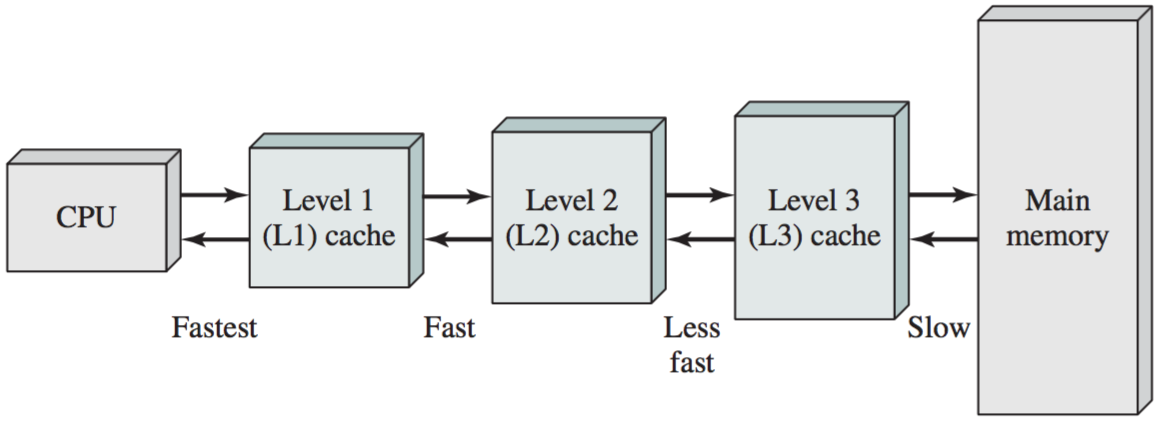
\includegraphics[width=0.6\textwidth]{images/caches.png}\\
Three levels of cache between the CPU and main memory.
\end{center}


\end{frame}



\begin{frame}
\frametitle{Pay Up}

Cliff Click said that 5\% miss rates dominate performance. Let's look at why.

Here are the reported cache miss rates for SPEC CPU2006.

\begin{center}
\begin{tabular}{ll}
L1D & 40 per 1000 \\
L2 & 4 per 1000
\end{tabular}
\end{center}

Let's assume that the L1D cache miss penalty is 5 cycles and the L2 miss penalty is
300 cycles, as in the video. 

Then, for every instruction, you would expect a running
time of, on average:
\[ 1 + 0.04 \times 5 + 0.004 \times 300 = 2.4. \]

\end{frame}



\begin{frame}
\frametitle{Bring in the Disk}

If we replace the terms $t_{c}$ and $t_{m}$ with $t_{m}$ and $t_{d}$ (time to retrieve it from disk) respectively, and redefine $h$ as $p$, the chance that a page is in memory.

Effective access time in virtual memory: 

\begin{center}
	Effective Access Time = $ p \times t_{m} + (1 - p) \times t_{d}$
\end{center}


\end{frame}



\begin{frame}
\frametitle{Put It Together}

We can combine the caching and disk read formulae to get the true effective access time for a system where there is only 1 level of cache:

\begin{center}
	Effective Access Time = $ h \times t_{c} + (1 - h) ( p \times t_{m} + (1 - p) \times t_{d})$
\end{center}

We can measure $t_{d}$ if we're so inclined.

\end{frame}



\begin{frame}
\frametitle{Slow as A Snail Chained to an Anvil}

The slow step is the amount of time it takes to load the page from disk. 

A typical hard drive in may have a latency of 3~ms, seek time is around 5~ms, and a transfer time of 0.05~ms. 

This is  several orders of magnitude larger than any of the other costs.

Several requests may be queued, making the time even longer.

\end{frame}



\begin{frame}
\frametitle{Dominating Flurry}


Thus the disk read term $t_{d}$ dominates the effective access time equation. 

We can roughly estimate the access time in nanoseconds as $(1-p) \times 8~000~000$. 

If the page fault rate is high, performance is awful. If performance of the computer is to be reasonable, the page fault rate has to be very, very low. 

On the order of $10^{-6}$. 

Summary: misses are not just expensive, they hurt performance so much.

\end{frame}



\begin{frame}
\frametitle{Predict and Mispredict}
The compiler (\& CPU) take a look at code that results in branch instructions.

Examples: loops, conditionals, or the dreaded \texttt{goto}.

It will take an assessment of what it thinks is likely to happen. 

\end{frame}



\begin{frame}
\frametitle{Let's Not Predict}

In the beginning the CPUs/compilers didn't really think about this sort of thing.

They come across instructions one at a time and do them and that was that. 

If one of them required a branch, it was no real issue. 

Then we had pipelining...
\end{frame}



\begin{frame}
\frametitle{Not Just for Oil}

the CPU would fetch the next instruction while decoding the previous one, and while executing the instruction before. 

That means if evaluation of an instruction results in a branch, we might go somewhere else and therefore throw away the contents of the pipeline. 

Thus we'd have wasted some time and effort. 

If the pipeline is short, this is not very expensive.\\
\quad But pipelines keep getting longer... 

\end{frame}



\begin{frame}
\frametitle{Take a Guess}

The compiler and CPU look at instructions on their way to be executed and analyze whether it thinks it's likely the branch is taken. 

This can be based on several things, including the recent execution history. 

If we guess correctly, this is great, because it minimizes the cost of the branch. 

If we guess wrong, we flush the pipeline and take the performance penalty.

\end{frame}



\begin{frame}
\frametitle{Take a Hint}

The compiler and CPU's branch prediction routines are pretty smart.\\
\quad Trying to outsmart them isn't necessarily a good idea. 

But we can give the compiler (\texttt{gcc} at least) some hints about what we think is likely to happen. 

Our tool for this is the \texttt{\_\_builtin\_expect()} function, which takes two arguments, the value to be tested and the expected result.

\end{frame}



\begin{frame}[fragile]
\frametitle{Check the Header}

In the linux \texttt{compiler.h} header there are two neat little shortcuts defined:

\begin{verbatim}
# define likely(x)      __builtin_expect(!!(x), 1)
# define unlikely(x)    __builtin_expect(!!(x), 0)
\end{verbatim}

Compile with at least optimization level 2 (\texttt{-O2}) to get the compiler to take these hints at all.

\end{frame}



\begin{frame}[fragile]
\frametitle{Force a Mispredict}
{\scriptsize
\begin{verbatim}
        #include <stdlib.h>
        #include <stdio.h>

        static __attribute__ ((noinline)) int f(int a) { return a; }

        #define BSIZE 1000000
        int main(int argc, char* argv[]) 
        {
          int *p = calloc(BSIZE, sizeof(int));
          int j, k, m1 = 0, m2 = 0;
          for (j = 0; j < 1000; j++) {
            for (k = 0; k < BSIZE; k++) {
              if (__builtin_expect(p[k], EXPECT_RESULT)) {
                m1 = f(++m1);
              } else {
                m2 = f(++m2);
              }
            }
          }

          printf("%d, %d\n", m1, m2);
        }
\end{verbatim}
}

\end{frame}



\begin{frame}[fragile]
\frametitle{Mispredict Results}

Running it yielded:
{\scriptsize
\begin{verbatim}
plam@plym:~/459$ gcc -O2 likely-simplified.c -DEXPECT_RESULT=0 -o likely-simplified
plam@plym:~/459$ time ./likely-simplified
0, 1000000000

real	0m2.521s
user	0m2.496s
sys	0m0.000s
plam@plym:~/459$ gcc -O2 likely-simplified.c -DEXPECT_RESULT=1 -o likely-simplified
plam@plym:~/459$ time ./likely-simplified
0, 1000000000

real	0m3.938s
user	0m3.868ss
sys	0m0.000s
\end{verbatim}
}
\end{frame}



\begin{frame}
\frametitle{Hint Results}

In the original source the author reports the following results.

Scanning a one million element array, with all elements initially zero, the results are:

\begin{itemize}
	\item No use of hints: \texttt{0:02.68 real,  2.67 user, 0.00 sys}
	\item Good prediction: \texttt{0:02.28 real,  2.28 user, 0.00 sys}
	\item Bad prediction: \texttt{0:04.19 real,  4.18 user, 0.00 sys}
\end{itemize}

When about one in ten thousand values in the array is nonzero, then it's roughly the ``break-even'' point for the setup as described.

Conclusion: it's hard to outsmart the compiler. Maybe it's better not to try.

\end{frame}


\begin{frame}
  \frametitle{Limitations of Speedups}

    Our main focus is parallelization.\\[1em]
  \begin{itemize}
    \item Most programs have a sequential part and a parallel part; and,\\[1em]
    \item Amdahl's Law answers, ``what are the limits to parallelization?''
  \end{itemize}

\end{frame}



\begin{frame}
\frametitle{Visualizing Amdahl's Law}

  \hspace*{2em}\begin{minipage}{.8\textwidth}
  $S$: fraction of serial runtime in a serial execution.

  $P$: fraction of parallel runtime in a serial execution.

  Therefore, $S + P = 1$.\\[2em]

  With 4 processors, best case, what can happen to the following runtime?
  \end{minipage}

  \hspace*{5em}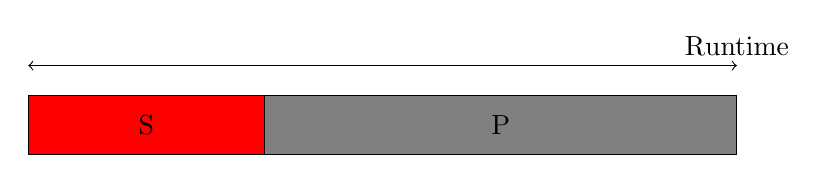
\begin{tikzpicture}
   \draw[<->] (-1.5,0.75) -- (7.5,0.75) node[above] {Runtime};
   \draw (0,0) node[rectangle, fill=red, minimum height=0.75cm, minimum width=3cm,draw] {S};
   \draw (4.5,0) node[rectangle, fill=gray, minimum height=0.75cm, minimum width=6cm,draw] {P};
  \end{tikzpicture}
\end{frame}

\begin{frame}
  \frametitle{Visualizing Amdahl's Law}

  \hspace*{5em}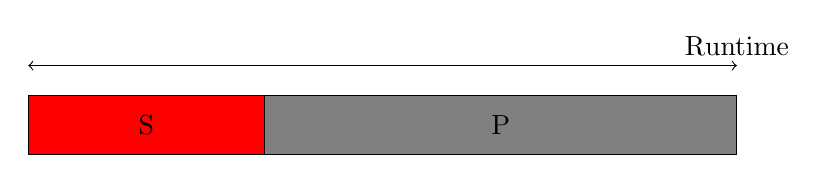
\begin{tikzpicture}
   \draw[<->] (-1.5,0.75) -- (7.5,0.75) node[above] {Runtime};
   \draw (0,0) node[rectangle, fill=red, minimum height=0.75cm, minimum width=3cm,draw] {S};
   \draw (4.5,0) node[rectangle, fill=gray, minimum height=0.75cm, minimum width=6cm,draw] {P};
  \end{tikzpicture}
  \vfill
  We want to split up the parallel part over 4 processors
  \vfill
  \hspace*{5em}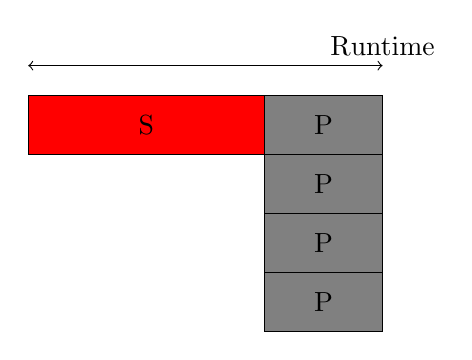
\begin{tikzpicture}
   \draw[<->] (-1.5,0.75) -- (3,0.75) node[above] {Runtime};
   \draw (0,0) node[rectangle, fill=red, minimum height=0.75cm, minimum width=3cm,draw] {S};
   \draw (2.25,0) node[rectangle, fill=gray, minimum height=0.75cm, minimum width=1.5cm,draw] {P};
   \draw (2.25,-0.75) node[rectangle, fill=gray, minimum height=0.75cm, minimum width=1.5cm,draw] {P};
   \draw (2.25,-1.5) node[rectangle, fill=gray, minimum height=0.75cm, minimum width=1.5cm,draw] {P};
   \draw (2.25,-2.25) node[rectangle, fill=gray, minimum height=0.75cm, minimum width=1.5cm,draw] {P};
  \end{tikzpicture}
\end{frame}

\begin{frame}
  \frametitle{Obey the Law}

\Large
$T_s$: time for the program to run in serial

$N$: number of processors/parallel executions

$T_p$: time for the program to run in parallel
\vfill
  \begin{itemize}
    \item Under perfect conditions, get $N$ speedup for $P$
  \end{itemize}
\vfill

  \begin{center}
$T_p = T_s \cdot (S + \frac{P}{N})$
  \end{center}
\end{frame}

\begin{frame}
  \frametitle{Obey the Law}

  \hspace*{3em} How much faster can we make the program?

  \begin{eqnarray*}
  \mbox{\em speedup} &=& \frac{T_s}{T_p}\\
                     &=& \frac{T_s}{T_S \cdot (S + \frac{P}{N})}\\
                     &=& \frac{1}{S + \frac{P}{N}}
  \end{eqnarray*}
  \vfill
  \hspace*{3em} (assuming no overhead for parallelizing; or costs near
  zero)

\end{frame}

\begin{frame}
  \frametitle{Fixed-Size Problem Scaling, \\ Varying Fraction of Parallel Code}

  \begin{center}
    \hspace*{2em}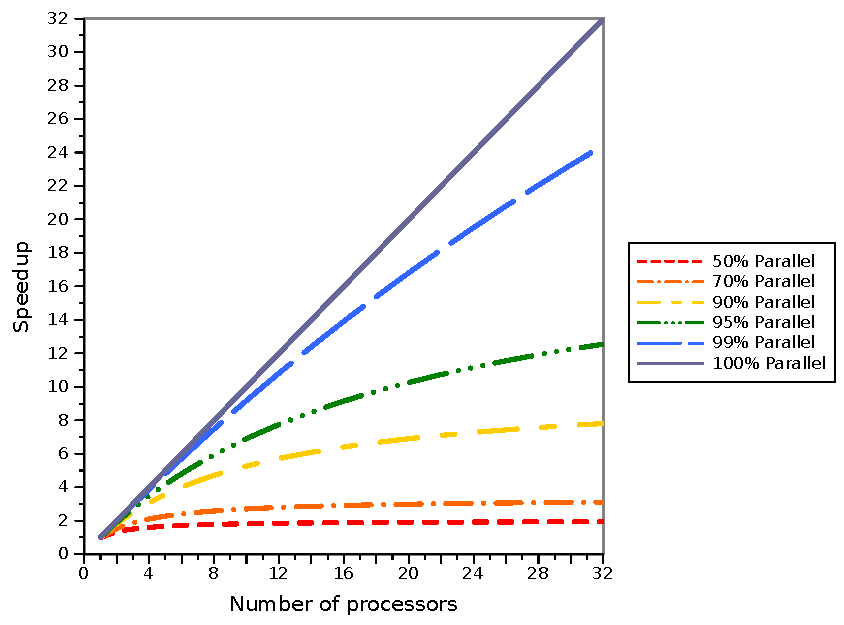
\includegraphics[scale=0.68]{images/parallel-scaling.pdf}
  \end{center}
\end{frame}


\begin{frame}
  \frametitle{Amdahl's Law}

 \hspace*{2em}Replace $S$ with $(1 - P)$:

  \begin{center}
    \structure{$\mbox{\em speedup} = \frac{1}{(1 - P) + \frac{P}{N}}$}
  \end{center}
  \vfill
  \begin{center}
    $\mbox{\em maximum speedup} = \frac{1}{(1 - P)}$, since $\frac{P}{N} \rightarrow 0$
  \end{center}

As you might imagine, the asymptotes in the previous graph are bounded by the
  maximum speedup.
\end{frame}

\begin{frame}
\frametitle{Speedup Example}


Suppose: a task that can be executed in 5~s, containing a parallelizable loop.

Initialization and recombination code in this routine requires 400~ms. 

So with one processor executing, it would take about 4.6~s to execute the loop. 

Split it up and execute on two processors: about 2.3~s to execute the loop. 

Add to that the setup and cleanup time of 0.4~s and we get a total time of 2.7~s. 

Completing the task in 2.7~s rather than 5~s represents a speedup of about~46\%.

\end{frame}


\begin{frame}
\frametitle{Amdahl's Law on the 5~s Task}

Applying this formula to the example:

\begin{center}
	\begin{tabular}{l|l}
	\textbf{Processors} & \textbf{Run Time (s)} \\ \hline
	1 & 5\\
	2 & 2.7\\
	4 & 1.55\\
	8 & 0.975\\
	16 & 0.6875 \\
	32 & 0.54375 \\
	64 & 0.471875 \\
	128 & 0.4359375\\
	\end{tabular}
\end{center}

\end{frame}

 
\begin{frame}
\frametitle{Observations on the 5~s Task}

1. Diminishing returns as we add more processors.

2. Converges on 0.4~s.

The most we could speed up this code is by a factor of $\frac{5}{0.4}\approx 12.5$.

But that would require infinite processors (and therefore infinite money).

\end{frame}

\begin{frame}
  \frametitle{Assumptions behind Amdahl's Law}

    We assume:
    \begin{itemize}
    \item problem size is fixed (we'll see this soon);
    \item program/algorithm behaves the same on 1 processor and on $N$ processors;
    \item that we can accurately measure runtimes---\\ ~~i.e. that overheads don't matter.
    \end{itemize}
  
\end{frame}

\begin{frame}
  \frametitle{Amdahl's Law Generalization}

  \hspace*{2em} The program may have many parts, each of which we can tune to
  a different degree.\\[1em]

  Let's generalize Amdahl's Law.\\[1em]

  $f_1, f_2, \ldots, f_n$: fraction of time in part $n$

  $S_{f_1}, S_{f_n}, \ldots, S_{f_n}$: speedup for part $n$

  \vfill
  \begin{center}
  \structure{\[\mbox{\em speedup} = \frac{1}{\frac{f_1}{S_{f_1}} + \frac{f_2}{S_{f_2}} + \ldots +
    \frac{f_n}{S_{f_n}}}\]}
  \end{center}
\end{frame}


\begin{frame}
  \frametitle{Application (1)}

  \hspace*{2em} 
Consider a program with 4 parts in the following scenario:\\[2em]
    \begin{tabular}{r|r|r|r}
    \multicolumn{2}{l}{} & \multicolumn{2}{c}{Speedup} \\
    Part & Fraction of Runtime & Option 1 & Option 2\\
    \hline
    1 & 0.55 & 1  & 2\\
    2 & 0.25 & 5  & 1\\
    3 & 0.15 & 3  & 1\\
    4 & 0.05  & 10 & 1\\
  \end{tabular}

~\\[2em]
  We can implement either Option 1 or Option 2. \\
  Which option is better?

\end{frame}

\begin{frame}
  \frametitle{Application (2)}


  \hspace*{2em} ``Plug and chug'' the numbers:\\[1em]

  {\bf Option 1} \vspace*{-2em}

  \[ \mbox{\em speedup} = \frac{1}{0.55 + \frac{0.25}{5} + \frac{0.15}{3} + \frac{0.05}{5}}
    = 1.53  \]
~\\[1em]
  {\bf Option 2} \vspace*{-2em}

   \[\mbox{\em speedup} = \frac{1}{\frac{0.55}{2} + 0.45} = 1.38 \hspace*{5.5em}\]


\end{frame}

\begin{frame}
  \frametitle{Empirically estimating parallel speedup P}

  \hspace*{2em} Useful to know, don't have to commit to memory:
  \vfill
  \[P_{\mbox{\scriptsize estimated}} = \frac{\frac{1}{\mbox{\em speedup}}-1}{\frac{1}{N}-1}\]
  \vfill
  \hspace*{2em} \begin{minipage}{.8\textwidth} \begin{itemize}
    \item Quick way to guess the fraction of parallel code
    \item Use $P_{\mbox{\scriptsize estimated}}$ to predict speedup for a different number of processors
  \end{itemize} \end{minipage}
\end{frame}

\begin{frame}
  \frametitle{Summary of Amdahl's Law}

\hspace*{2em} Important to focus on the part of the program with most impact.\\[1em]

\hspace*{2em} Amdahl's Law:\\[1em]
\hspace*{2em}
  \begin{itemize}
    \item estimates perfect performance gains from
          parallelization (under assumptions); but,
    \vfill
    \item only applies to solving a \structure{fixed problem size} in the
          shortest possible period of time
  \end{itemize}
\end{frame}

\begin{frame}
  \frametitle{Gustafson's Law: Formulation}

\hspace*{2em} 
\begin{tabbing}
  $n$:~~~~~~ \= problem size\\[.1em]

  $S(n)$: \> fraction of serial runtime for a parallel execution\\[.1em]

  $P(n)$: \> fraction of parallel runtime for a parallel execution\\
\end{tabbing}


\begin{eqnarray*}
T_p &=& S(n) + P(n) = 1 \\
T_s &=& S(n) + N \cdot P(n) 
\end{eqnarray*}

\[ \mbox{\em speedup} = \frac{T_s}{T_p} \]
\end{frame}

\begin{frame}
  \frametitle{Gustafson's Law}

\hspace*{2em}
  \structure{$speedup = S(n) + N \cdot P(n)$}\\[1em]

  Assuming the fraction of runtime in serial part decreases as $n$ increases,
  the speedup approaches $N$.


Yes! Large problems can be efficiently parallelized. (Ask Google.)

\end{frame}

\begin{frame}
  \frametitle{Driving Metaphor}

  {\bf Amdahl's Law}
  
  Suppose you're travelling between 2 cities 90~km apart. If you travel for an
  hour at a constant speed less than 90 km/h, your average will never equal
  90~km/h, even if you energize after that hour.
  \vfill
  {\bf Gustafson's Law}

  Suppose you've been travelling at a constant speed less than 90~km/h. Given
  enough distance, you can bring your average up to 90~km/h.
\end{frame}

\end{document}

